\documentclass[]{article}
\usepackage{lmodern}
\usepackage{amssymb,amsmath}
\usepackage{ifxetex,ifluatex}
\usepackage{fixltx2e} % provides \textsubscript
\ifnum 0\ifxetex 1\fi\ifluatex 1\fi=0 % if pdftex
  \usepackage[T1]{fontenc}
  \usepackage[utf8]{inputenc}
\else % if luatex or xelatex
  \ifxetex
    \usepackage{mathspec}
  \else
    \usepackage{fontspec}
  \fi
  \defaultfontfeatures{Ligatures=TeX,Scale=MatchLowercase}
\fi
% use upquote if available, for straight quotes in verbatim environments
\IfFileExists{upquote.sty}{\usepackage{upquote}}{}
% use microtype if available
\IfFileExists{microtype.sty}{%
\usepackage{microtype}
\UseMicrotypeSet[protrusion]{basicmath} % disable protrusion for tt fonts
}{}
\usepackage[margin=1in]{geometry}
\usepackage{hyperref}
\hypersetup{unicode=true,
            pdftitle={TP6\_Analysis\_Dejous},
            pdfauthor={Alexandre Dejous},
            pdfborder={0 0 0},
            breaklinks=true}
\urlstyle{same}  % don't use monospace font for urls
\usepackage{color}
\usepackage{fancyvrb}
\newcommand{\VerbBar}{|}
\newcommand{\VERB}{\Verb[commandchars=\\\{\}]}
\DefineVerbatimEnvironment{Highlighting}{Verbatim}{commandchars=\\\{\}}
% Add ',fontsize=\small' for more characters per line
\usepackage{framed}
\definecolor{shadecolor}{RGB}{248,248,248}
\newenvironment{Shaded}{\begin{snugshade}}{\end{snugshade}}
\newcommand{\KeywordTok}[1]{\textcolor[rgb]{0.13,0.29,0.53}{\textbf{#1}}}
\newcommand{\DataTypeTok}[1]{\textcolor[rgb]{0.13,0.29,0.53}{#1}}
\newcommand{\DecValTok}[1]{\textcolor[rgb]{0.00,0.00,0.81}{#1}}
\newcommand{\BaseNTok}[1]{\textcolor[rgb]{0.00,0.00,0.81}{#1}}
\newcommand{\FloatTok}[1]{\textcolor[rgb]{0.00,0.00,0.81}{#1}}
\newcommand{\ConstantTok}[1]{\textcolor[rgb]{0.00,0.00,0.00}{#1}}
\newcommand{\CharTok}[1]{\textcolor[rgb]{0.31,0.60,0.02}{#1}}
\newcommand{\SpecialCharTok}[1]{\textcolor[rgb]{0.00,0.00,0.00}{#1}}
\newcommand{\StringTok}[1]{\textcolor[rgb]{0.31,0.60,0.02}{#1}}
\newcommand{\VerbatimStringTok}[1]{\textcolor[rgb]{0.31,0.60,0.02}{#1}}
\newcommand{\SpecialStringTok}[1]{\textcolor[rgb]{0.31,0.60,0.02}{#1}}
\newcommand{\ImportTok}[1]{#1}
\newcommand{\CommentTok}[1]{\textcolor[rgb]{0.56,0.35,0.01}{\textit{#1}}}
\newcommand{\DocumentationTok}[1]{\textcolor[rgb]{0.56,0.35,0.01}{\textbf{\textit{#1}}}}
\newcommand{\AnnotationTok}[1]{\textcolor[rgb]{0.56,0.35,0.01}{\textbf{\textit{#1}}}}
\newcommand{\CommentVarTok}[1]{\textcolor[rgb]{0.56,0.35,0.01}{\textbf{\textit{#1}}}}
\newcommand{\OtherTok}[1]{\textcolor[rgb]{0.56,0.35,0.01}{#1}}
\newcommand{\FunctionTok}[1]{\textcolor[rgb]{0.00,0.00,0.00}{#1}}
\newcommand{\VariableTok}[1]{\textcolor[rgb]{0.00,0.00,0.00}{#1}}
\newcommand{\ControlFlowTok}[1]{\textcolor[rgb]{0.13,0.29,0.53}{\textbf{#1}}}
\newcommand{\OperatorTok}[1]{\textcolor[rgb]{0.81,0.36,0.00}{\textbf{#1}}}
\newcommand{\BuiltInTok}[1]{#1}
\newcommand{\ExtensionTok}[1]{#1}
\newcommand{\PreprocessorTok}[1]{\textcolor[rgb]{0.56,0.35,0.01}{\textit{#1}}}
\newcommand{\AttributeTok}[1]{\textcolor[rgb]{0.77,0.63,0.00}{#1}}
\newcommand{\RegionMarkerTok}[1]{#1}
\newcommand{\InformationTok}[1]{\textcolor[rgb]{0.56,0.35,0.01}{\textbf{\textit{#1}}}}
\newcommand{\WarningTok}[1]{\textcolor[rgb]{0.56,0.35,0.01}{\textbf{\textit{#1}}}}
\newcommand{\AlertTok}[1]{\textcolor[rgb]{0.94,0.16,0.16}{#1}}
\newcommand{\ErrorTok}[1]{\textcolor[rgb]{0.64,0.00,0.00}{\textbf{#1}}}
\newcommand{\NormalTok}[1]{#1}
\usepackage{graphicx,grffile}
\makeatletter
\def\maxwidth{\ifdim\Gin@nat@width>\linewidth\linewidth\else\Gin@nat@width\fi}
\def\maxheight{\ifdim\Gin@nat@height>\textheight\textheight\else\Gin@nat@height\fi}
\makeatother
% Scale images if necessary, so that they will not overflow the page
% margins by default, and it is still possible to overwrite the defaults
% using explicit options in \includegraphics[width, height, ...]{}
\setkeys{Gin}{width=\maxwidth,height=\maxheight,keepaspectratio}
\IfFileExists{parskip.sty}{%
\usepackage{parskip}
}{% else
\setlength{\parindent}{0pt}
\setlength{\parskip}{6pt plus 2pt minus 1pt}
}
\setlength{\emergencystretch}{3em}  % prevent overfull lines
\providecommand{\tightlist}{%
  \setlength{\itemsep}{0pt}\setlength{\parskip}{0pt}}
\setcounter{secnumdepth}{0}
% Redefines (sub)paragraphs to behave more like sections
\ifx\paragraph\undefined\else
\let\oldparagraph\paragraph
\renewcommand{\paragraph}[1]{\oldparagraph{#1}\mbox{}}
\fi
\ifx\subparagraph\undefined\else
\let\oldsubparagraph\subparagraph
\renewcommand{\subparagraph}[1]{\oldsubparagraph{#1}\mbox{}}
\fi

%%% Use protect on footnotes to avoid problems with footnotes in titles
\let\rmarkdownfootnote\footnote%
\def\footnote{\protect\rmarkdownfootnote}

%%% Change title format to be more compact
\usepackage{titling}

% Create subtitle command for use in maketitle
\providecommand{\subtitle}[1]{
  \posttitle{
    \begin{center}\large#1\end{center}
    }
}

\setlength{\droptitle}{-2em}

  \title{TP6\_Analysis\_Dejous}
    \pretitle{\vspace{\droptitle}\centering\huge}
  \posttitle{\par}
    \author{Alexandre Dejous}
    \preauthor{\centering\large\emph}
  \postauthor{\par}
      \predate{\centering\large\emph}
  \postdate{\par}
    \date{5/17/2019}


\begin{document}
\maketitle

\section{Part A: Stationnary
Analysis}\label{part-a-stationnary-analysis}

\subsection{Question 1 and 2:}\label{question-1-and-2}

\begin{Shaded}
\begin{Highlighting}[]
\KeywordTok{setwd}\NormalTok{(}\StringTok{"C:/Users/Alexandre/Desktop/A2/Analyse/TP6_Analysis"}\NormalTok{)}
\KeywordTok{library}\NormalTok{(tseries)}
\KeywordTok{data}\NormalTok{(USeconomic)}
\NormalTok{logGNP =}\StringTok{ }\KeywordTok{as.vector}\NormalTok{(USeconomic[,}\DecValTok{2}\NormalTok{])}
\NormalTok{year =}\StringTok{ }\KeywordTok{seq}\NormalTok{(}\DecValTok{1954}\NormalTok{,}\FloatTok{1987.75}\NormalTok{,}\FloatTok{0.25}\NormalTok{)}
\NormalTok{DATA =}\StringTok{ }\KeywordTok{data.frame}\NormalTok{(year,logGNP)}
\KeywordTok{plot}\NormalTok{(DATA}\OperatorTok{$}\NormalTok{year, DATA}\OperatorTok{$}\NormalTok{logGNP)}
\end{Highlighting}
\end{Shaded}

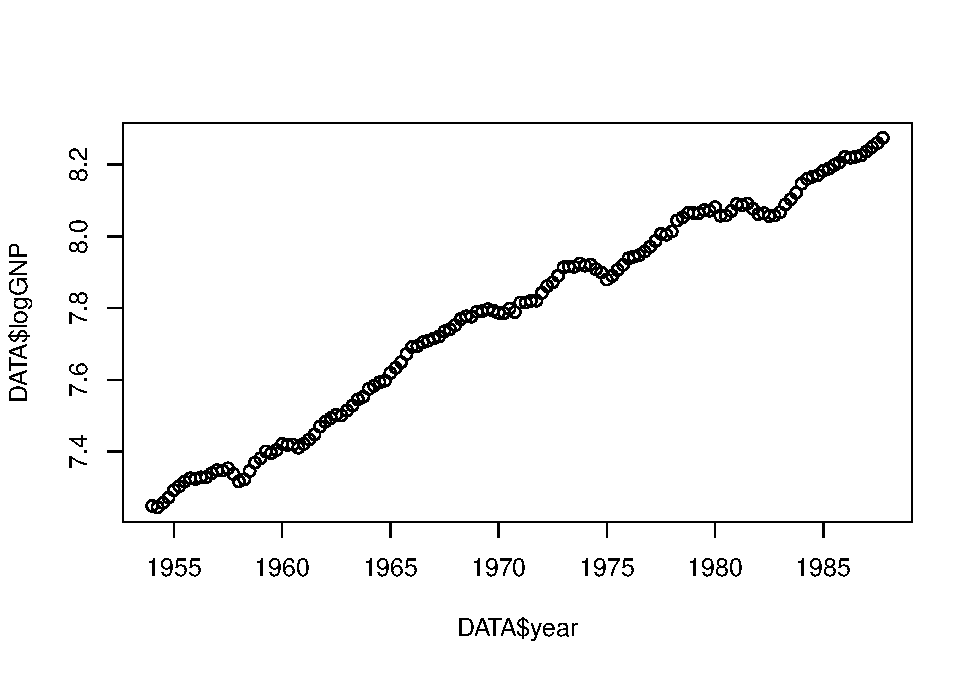
\includegraphics{TP6_Analysis_Dejous_files/figure-latex/unnamed-chunk-1-1.pdf}

\subsection{Question 3}\label{question-3}

In a stationnary time serie, the ensemble mean and thetime average of a
sample path are approximately equal. For a strict stationnary time
serie, all the observations are drawn from the same distribution, for a
weak stationnary time serie, we expect only the observations to come
from distributions with the same mean, variance and covariance. In the
plot we just drew, we visually assess that the samples values increase
gradually on average on a significant number of samples, which should
not happen if the samples were taken from the same distribution. We
conclude that the time serie is not stationnary.

\subsection{Question 4}\label{question-4}

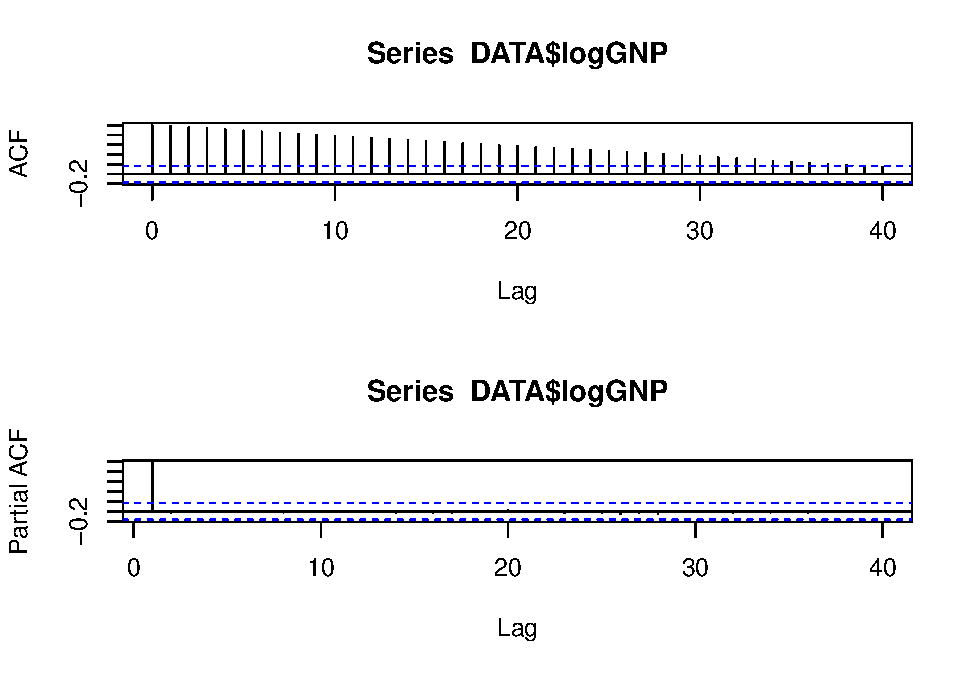
\includegraphics{TP6_Analysis_Dejous_files/figure-latex/unnamed-chunk-2-1.pdf}

It seems that tha ACF is steadily decreasing, which could indicate that
logGNP follows a trend. The PACF indicates us that this trend can be
modeled with an auto regressive model of order 1.

\subsection{Question 5:}\label{question-5}

\begin{verbatim}
## 
##  Box-Pierce test
## 
## data:  DATA$logGNP
## X-squared = 129.98, df = 1, p-value < 2.2e-16
\end{verbatim}

The null hypothesis of this test stipulates that there is no
auto-correlation between the values taken by our data. However, since
our p value is very close to 0, we reject this null hypothesis and have
confirmation that our data follows and trend and is not just white
noise.

\subsection{Question 6:}\label{question-6}

As is (not derived) our time series is not stationnary. It follows a
trend and its samples are not taken from an iid distribution, as shown
by the bow pierce test.

\section{PART B:}\label{part-b}

\subsection{Question 1 and 2}\label{question-1-and-2-1}

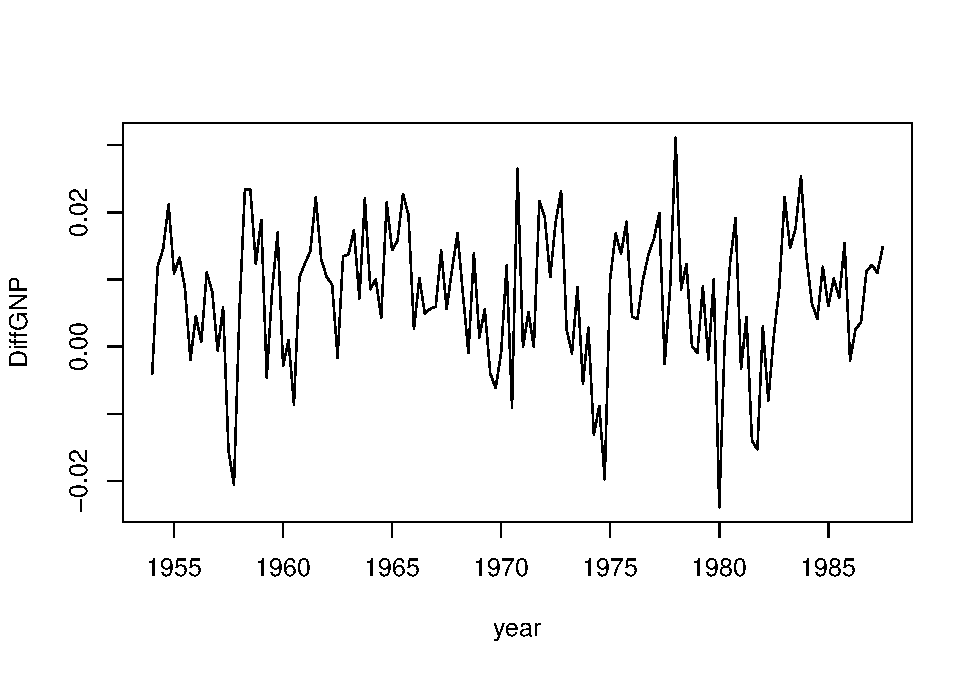
\includegraphics{TP6_Analysis_Dejous_files/figure-latex/unnamed-chunk-4-1.pdf}

This time series represents the variation between two consecutive
samples at time t (diff between t+1 and t).

\subsection{Question 3:}\label{question-3-1}

\begin{verbatim}
## 
##  One Sample t-test
## 
## data:  DiffGNP
## t = 8.6739, df = 134, p-value = 1.223e-14
## alternative hypothesis: true mean is not equal to 0
## 95 percent confidence interval:
##  0.005864407 0.009328764
## sample estimates:
##   mean of x 
## 0.007596586
\end{verbatim}

This student test supports the following null hypothesis: the value of
the mean is not equal to 0. In fact, the true mean should be a positive
value, as shows the IC95, which is coherent with our previous results :
the original time series follows a trend and this trend seems to be
positive.

\subsection{Question 4:}\label{question-4-1}

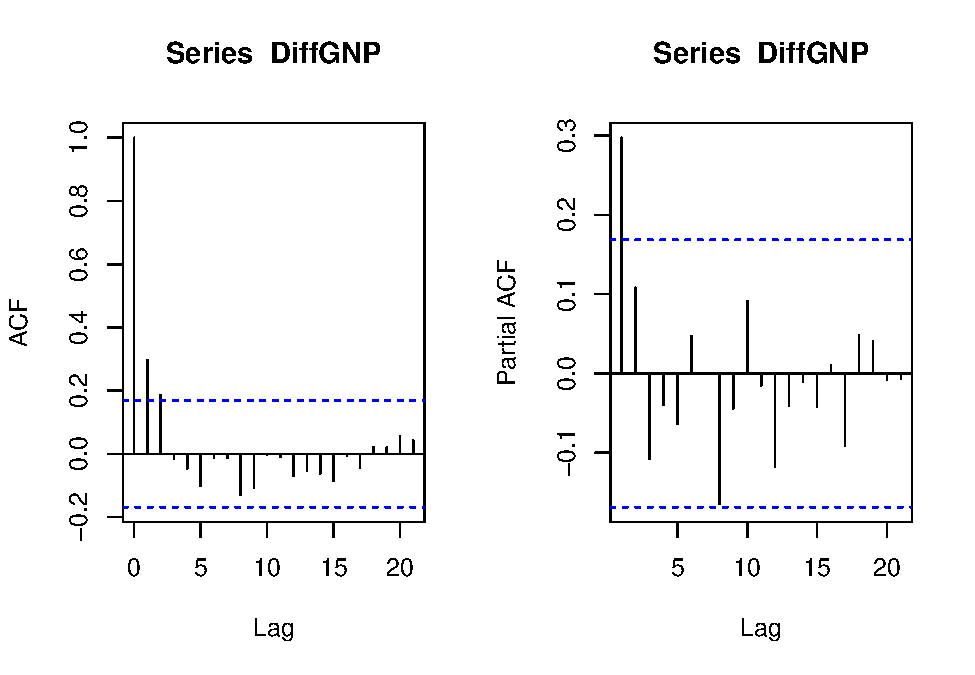
\includegraphics{TP6_Analysis_Dejous_files/figure-latex/unnamed-chunk-6-1.pdf}

The ACF shows us that the q parameter of our arma model might be 1 or 2,
while the p parameter determined by the PACF might be 0 or 8. Our ARMA
model might be ARMA(0,1), ARMA(8,1), ARMA(0,2) or ARMA(8,2).

\subsection{Question 5:}\label{question-5-1}

\begin{verbatim}
## [1] "---------------0,1---------------"
\end{verbatim}

\begin{verbatim}
## $loglik
## [1] 433.0268
## 
## $aic
## [1] -860.0536
\end{verbatim}

\begin{verbatim}
## [1] "---------------8,1---------------"
\end{verbatim}

\begin{verbatim}
## $loglik
## [1] 438.4921
## 
## $aic
## [1] -854.9841
\end{verbatim}

\begin{verbatim}
## [1] "---------------0,2---------------"
\end{verbatim}

\begin{verbatim}
## $loglik
## [1] 435.8643
## 
## $aic
## [1] -863.7286
\end{verbatim}

\begin{verbatim}
## [1] "---------------8,2---------------"
\end{verbatim}

\begin{verbatim}
## $loglik
## [1] 439.6611
## 
## $aic
## [1] -855.3222
\end{verbatim}

The log likelihood gives us a measure of fitness for our model, the
higher the better. The AIC gives a measure of fitness and evaluates the
simplicity of our model at the same time. The simplest and fittest model
minimizes the AIC index. If we only look at the log likelihood, it seems
that the model ARMA(8,2) is the best. However, when comparing the two
model with the AIC, the AIC indicates us that we should choose the model
ARMA(0,2), because it has less parameters.

\subsection{Question 6:}\label{question-6-1}

If the residuals follow a trend, it means that our model could fit
better the samples, if they don't, it means that our model perfectly
fits the samples and is adapted. We do the Box-Pierce test and
Shapiro-Wilk test on the residuals of our ARMA model applied to DiffGNP
for these coefficients : arma(0,1), arma(0,2) and arma(8,2) The null
hypothesis of the Box-Pierce test states that there is no
autocorrelation in the data, while the null hypothesis of the
Shapiro-Wilk test states that the samples came from a normally
distributed population. To ensure that our model has the best accuracy
possible, we must make sure that the residuals don't follow a trend, and
that they're normally distributed. Thus, we need to check that the
p-value of both test does not reject the null hypothesis
(p\textgreater{} 0.05), we can also compare the models between them.

\begin{verbatim}
## [1] "---------------0,1---------------"
\end{verbatim}

\begin{verbatim}
## 
##  Box-Pierce test
## 
## data:  model0_1
## X-squared = 0.28287, df = 1, p-value = 0.5948
\end{verbatim}

\begin{verbatim}
## 
##  Shapiro-Wilk normality test
## 
## data:  model0_1
## W = 0.97756, p-value = 0.02493
\end{verbatim}

\begin{verbatim}
## [1] "---------------0,2---------------"
\end{verbatim}

\begin{verbatim}
## 
##  Box-Pierce test
## 
## data:  model0_2
## X-squared = 0.0043454, df = 1, p-value = 0.9474
\end{verbatim}

\begin{verbatim}
## 
##  Shapiro-Wilk normality test
## 
## data:  model0_2
## W = 0.98847, p-value = 0.3231
\end{verbatim}

\begin{verbatim}
## [1] "---------------8,2---------------"
\end{verbatim}

\begin{verbatim}
## 
##  Box-Pierce test
## 
## data:  model8_2
## X-squared = 1.3959e-07, df = 1, p-value = 0.9997
\end{verbatim}

\begin{verbatim}
## 
##  Shapiro-Wilk normality test
## 
## data:  model8_2
## W = 0.98606, p-value = 0.1872
\end{verbatim}

The box pierce test indicates that there is a higher suspicion for a
trend for model (0,1) rather than the two other model, whose p-values
are close to 1. The shapiro wilk test indicates that the model (0,1) did
not come from a normally distributed population, while for the two other
models H0 still holds.

It would be useful to display the aurocorrelogram of the residuals, in
order to see if the residuals of a model can themselves be described by
another model. Indeed, we obtain these results:

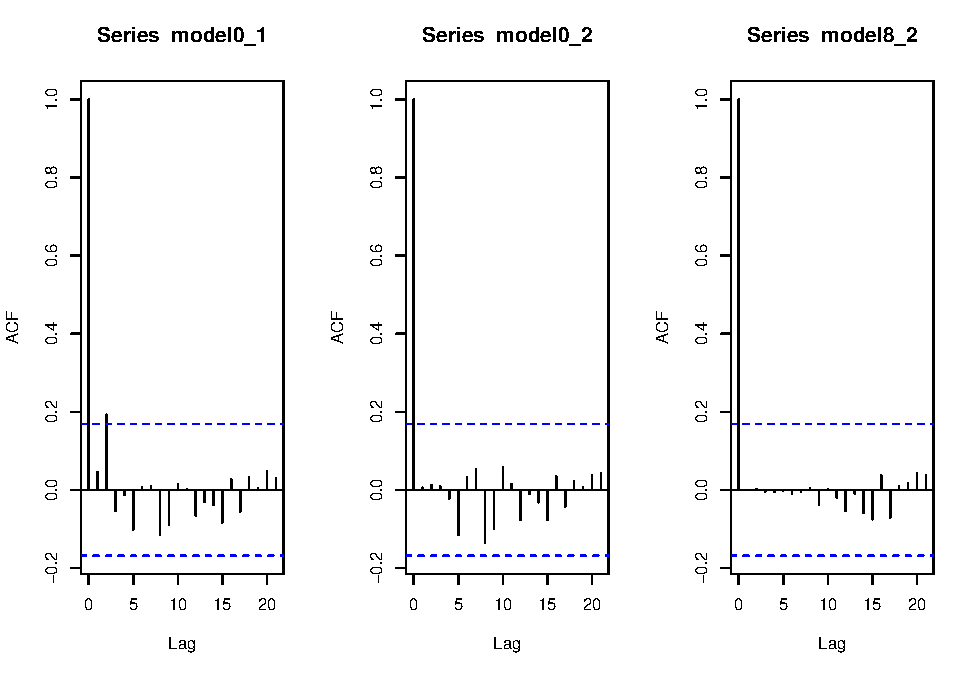
\includegraphics{TP6_Analysis_Dejous_files/figure-latex/unnamed-chunk-9-1.pdf}

We cannot seem to make sense of a model for (0,2) and (8,2), however,
the acf of the residuals of (0,1) indicates that these can be modeled by
a MA(2). The model (0,1) lacks accuracy, we can definetly direct our
attention to the two other models.

Having to choose between (0,2) and (8,2), we decide to


\end{document}
